\حصہ{ہذلولی تفاعل}
ہر ایسا تفاعل \عددی{f} جس کے دائرہ کار کا وسط مبدا پر واقع ہو کو ایک جفت اور ایک طاق تفاعل کا مجموعہ لکھا جا سکتا ہے:
\begin{align*}
f(x)=\underbrace{\frac{f(x)+f(-x)}{2}}_{\text{\RL{جفت حصہ}}}+\underbrace{\frac{f(x)-f(-x)}{2}}_{\text{\RL{طاق حصہ}}}
\end{align*}
یوں قوت نمائی تفاعل \عددی{e^x} کو درج ذیل لکھا جا سکتا ہے۔
\begin{align*}
e^x=\underbrace{\frac{e^x+e^{-x}}{2}}_{\text{\RL{جفت حصہ}}}+\underbrace{\frac{e^x-e^{-x}}{2}}_{\text{\RL{طاق حصہ}}}
\end{align*} 
قوت نمائی تفاعل \عددی{e^x} کا جفت اور طاق حصہ، جنہیں  بالترتیب \عددی{x} کا ہذلولی کوسائن اور ہذلولی سائن کہتے ہیں، از خود اہمیت کے حامل ہیں۔ یہ لچکدار ٹھوس مادہ میں لہروں کی حرکت، کھمبوں کے بیچ برقی تاروں کا روپ، اور دھاتی \اصطلاح{سرد کار}\حاشیہب{heat sink} میں حرارتی کی تقسیم کو بیان کرتے ہیں۔

\جزوحصہء{تعریف اور تماثل}
ہذلولی کوسائن اور ہذلولی سائن کی تعریف جدول \حوالہ{جدول_ماورائی_چھ_بنیادی_ہذلولی_تفاعل} کی پہلی دو مساواتیں پیش کرتی ہیں۔ اس جدول میں ہذلولی ٹینجنٹ، ہذلولی کوٹینجنٹ، ہذلولی سیکنٹ، اور ہذلولی کوسیکنٹ کی تعریف بھی پیش کی گئی ہیں۔ جیسا کہ ہم دیکھیں گے، ہذلولی تفاعل ان تکونیاتی تفاعل کے ساتھ کافی  ملتے جلتے ہیں جن کے توسط سے ان کے نام رکھے گئے ہیں۔ ان کو شکل \حوالہ{شکل_ماورائی_چھ_بنیادی_ہذلولی_تفاعل} میں ترسیم کیا گیا ہے۔

\begin{table}
\caption{چھ بنیادی ہذلولی تفاعل}
\label{جدول_ماورائی_چھ_بنیادی_ہذلولی_تفاعل}
\centering
\renewcommand{\arraystretch}{2.5}
\begin{tabular}{rl}
\toprule
\عددی{x} کا ہذلولی کوسائن& \عددی{\cosh=\dfrac{e^x+e^{-x}}{2}}\\
\عددی{x} کا ہذلولی سائن & \عددی{\sinh x=\dfrac{e^x-e^{-x}}{2}}\\
\عددی{x} کا ہذلولی ٹینجنٹ&\عددی{\tanh x=\dfrac{\sinh x}{\cosh x}=\dfrac{e^x-e^{-x}}{e^x+e^{-x}}}\\
\عددی{x} کا ہذلولی کوٹینجنٹ&\عددی{\coth x=\dfrac{\cosh x}{\sinh x}=\dfrac{e^x+e^{-x}}{e^x-e^{-x}}}\\
\عددی{x} کا ہذلولی سیکنٹ&\عددی{\sech x=\dfrac{1}{\cosh x}=\dfrac{2}{e^x+e^{-x}}}\\
\عددی{x} کا ہذلولی کوسیکنٹ&\عددی{\csch x=\dfrac{1}{\sinh x}=\dfrac{2}{e^x-e^{-x}}}\\
\bottomrule
\end{tabular}
\end{table}

\begin{figure}
\centering
\begin{subfigure}{0.45\textwidth}
\centering
\begin{tikzpicture}[font=\small,declare function={f(\x)=sinh(\x);g(\x)=1/2*e^(\x);k(\x)=-1/2*e^(-\x);}]
\begin{axis}[clip=false,small,axis lines=middle,xlabel={$x$},ylabel={$y$},xlabel style={at={(current axis.right of origin)},anchor=west},ylabel style={at={(current axis.above origin)},anchor=south},enlargelimits=true]
\addplot[domain=-2:2]{f(x)}node[pos=0.75,below right]{$y=\sinh x$};
\addplot[domain=-2:2]{g(x)}node[pos=0.75,above left]{$y=\dfrac{e^x}{2}$};
\addplot[domain=-2:2]{k(x)}node[pos=0.75,below right,yshift=-2ex]{$y=-\dfrac{e^{-x}}{2}$};
\end{axis}
\end{tikzpicture}
\caption{ہذلولی سائن اور اس کے قوت نما اجزاء۔}
\end{subfigure}\hfill
\begin{subfigure}{0.45\textwidth}
\centering
\begin{tikzpicture}[font=\small,declare function={f(\x)=cosh(\x);g(\x)=1/2*e^(\x);k(\x)=1/2*e^(-\x);}]
\begin{axis}[clip=false,small,axis lines=middle,xlabel={$x$},ylabel={$y$},xlabel style={at={(current axis.right of origin)},anchor=west},ylabel style={at={(current axis.above origin)},anchor=south},enlargelimits=true]
\addplot[domain=-2:2]{f(x)}node[pos=0.85,left]{$y=\cosh x$};
\addplot[domain=-2:2]{g(x)}node[pos=0.75,below right]{$y=\dfrac{e^x}{2}$};
\addplot[domain=-2:2]{k(x)}node[pos=0.25,below left]{$y=\dfrac{e^{-x}}{2}$};
\end{axis}
\end{tikzpicture}
\caption{ہذلولی کوسائن اور اس کے قوت نما اجزاء۔}
\end{subfigure}
\begin{subfigure}{0.45\textwidth}
\centering
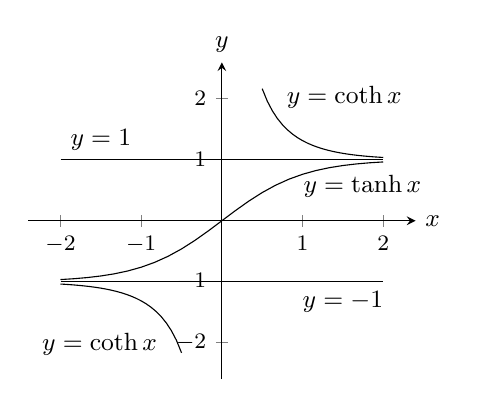
\begin{tikzpicture}[font=\small,declare function={f(\x)=tanh(\x);g(\x)=1/tanh(\x);}]
\begin{axis}[clip=false,small,axis lines=middle,xlabel={$x$},ylabel={$y$},xlabel style={at={(current axis.right of origin)},anchor=west},ylabel style={at={(current axis.above origin)},anchor=south},enlargelimits=true]
\addplot[domain=-2:2]{f(x)}node[pos=0.75,below right,yshift=1ex]{$y=\tanh x$};
\addplot[domain=0.5:2]{g(x)}node[pos=0.25,above right]{$y=\coth x$};
\addplot[domain=-0.5:-2]{g(x)}node[pos=0.25,below left]{$y=\coth x$};
\draw(-2,1)--(2,1)  (-2,-1)--(2,-1);
\draw(-1.5,1)node[above]{$y=1$}  (1.5,-1)node[below]{$y=-1$};
\end{axis}
\end{tikzpicture}
\caption{ہذلولی ٹینجنٹ اور ہذلولی کوٹینجنٹ۔}
\end{subfigure}\hfill
\begin{subfigure}{0.45\textwidth}
\centering
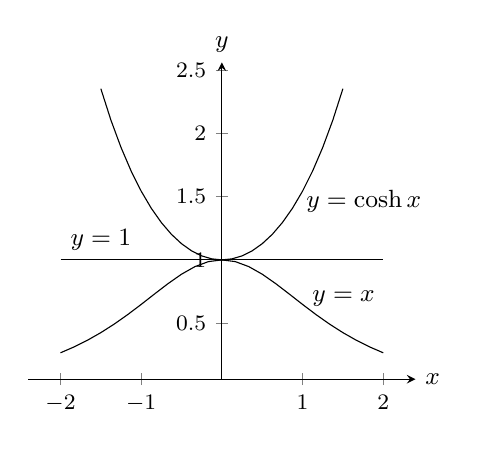
\begin{tikzpicture}[font=\small,declare function={f(\x)=cosh(\x);g(\x)=1/cosh(\x);}]
\begin{axis}[clip=false,small,axis lines=middle,xlabel={$x$},ylabel={$y$},xlabel style={at={(current axis.right of origin)},anchor=west},ylabel style={at={(current axis.above origin)},anchor=south},enlargelimits=true]
\addplot[domain=-1.5:1.5]{f(x)}node[pos=0.75,right]{$y=\cosh x$};
\addplot[domain=-2:2]{g(x)}node[pos=0.75,above right,yshift=-1ex]{$y=\sech x$};
\draw(-2,1)--(2,1);
\draw(-1.5,1)node[above]{$y=1$};
\end{axis}
\end{tikzpicture}
\caption{ہذلولی کوسائن اور ہذلولی سیکنٹ۔}
\end{subfigure}
\begin{subfigure}{0.45\textwidth}
\centering
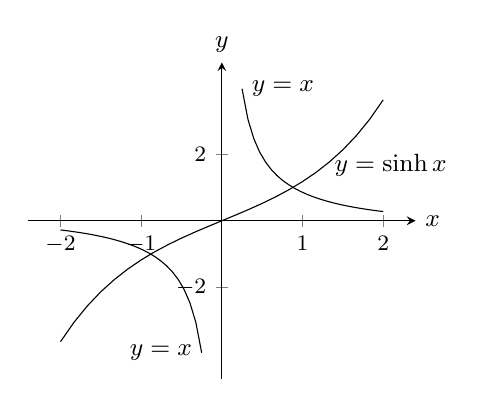
\begin{tikzpicture}[font=\small,declare function={f(\x)=sinh(\x);g(\x)=1/sinh(\x);}]
\begin{axis}[clip=false,small,axis lines=middle,xlabel={$x$},ylabel={$y$},xlabel style={at={(current axis.right of origin)},anchor=west},ylabel style={at={(current axis.above origin)},anchor=south},enlargelimits=true,ytick={-2,2}]
\addplot[domain=-2:2]{f(x)}node[pos=0.75,right]{$y=\sinh x$};
\addplot[domain=0.25:2]{g(x)}node[pos=0,right]{$y=\csch x$};
\addplot[domain=-0.25:-2]{g(x)}node[pos=0,left]{$y=\csch x$};
\end{axis}
\end{tikzpicture}
\caption{ہذلولی سائن اور ہذلولی کوسیکنٹ۔}
\end{subfigure}
\caption{چھ بنیادی ہذلولی تفاعل۔}
\label{شکل_ماورائی_چھ_بنیادی_ہذلولی_تفاعل}
\end{figure}

\جزوحصہء{تماثل}
ہذلولی تفاعل جدول \حوالہ{جدول_ماورائی_تماثل} میں دی گئی تماثل کو مطمئن کرتے ہیں۔ ماسوائے علامت، ہم ان تماثل کو تکونیاتی تفاعل سے جانتے ہیں۔

\begin{table}
\caption{ہذلولی تفاعل کے تماثل۔}
\label{جدول_ماورائی_تماثل}
\centering
\renewcommand{\arraystretch}{2}
\begin{tabular}{L}
\toprule
\sinh2x=2\sinh x \cosh x\\
\cosh2x=\cosh^2x+\sinh^2x\\
\cosh^2x=\dfrac{\cosh 2x+1}{2}\\
\sinh^2x=\dfrac{\cosh 2x-1}{2}\\
\cosh^2x-\sinh^2=1\\
\tanh^2x=1-\sech^2x\\
\coth^2x=1+\csch^2x\\
\bottomrule
\end{tabular}
\end{table} 

\جزوحصہء{تفرق اور تکمل}
چھ بنیادی ہذلولی تفاعل، قابل تفرق تفاعل \عددی{e^x} اور \عددی{e^{-x}} کے ناطق مجموعے ہیں، لہٰذا یہ ہر اس نقطہ پر قابل تفرق ہوں گے  جس پر یہ معین ہوں۔ یہاں بھی تکونیاتی تفاعل کے ساتھ مشابہت نظر آتی ہے۔ جدول \حوالہ{جدول_ماورائی_ہذلولی_کلیات_تفرق_تکمل}-ا کے کلیات تفرق سے جدول \حوالہ{جدول_ماورائی_ہذلولی_کلیات_تفرق_تکمل}-ب کے کلیات تکمل حاصل ہوتے ہیں۔ تکونیاتی تفاعل کی طرح ہذلولی تفاعل کی قیمتوں  کو بھی کیلکولیٹر سے حاصل کیا جا سکتا ہے۔

\begin{table}
\caption{ہذلولی تفاعل کے کلیات تفرق اور کلیات تکمل۔}
\label{جدول_ماورائی_ہذلولی_کلیات_تفرق_تکمل}
\centering
\renewcommand{\arraystretch}{2}
\begin{subtable}{0.45\textwidth}
\caption{ہذلولی تفاعل کے تفرق۔}
\centering
\begin{tabular}{L}
\toprule
\frac{\dif}{\dif x}(\sinh u)=\cosh u\frac{\dif u}{\dif x}\\
\frac{\dif}{\dif x}(\cosh u)=\sinh u\frac{\dif u}{\dif x}\\
\frac{\dif}{\dif x}(\tanh u)=\sech^2 u\frac{\dif u}{\dif x}\\
\frac{\dif}{\dif x}(\coth u)=-\csch^2 u\frac{\dif u}{\dif x}\\
\frac{\dif}{\dif x}(\sech u)=-\sech u\tanh u \frac{\dif u}{\dif x}\\
\frac{\dif}{\dif x}(\csch u)=-\csch u\coth u\frac{\dif u}{\dif x}\\
\bottomrule
\end{tabular}
\end{subtable}\hfill
\begin{subtable}{0.45\textwidth}
\caption{ہذلولی تفاعل کے تکمل۔}
\centering
\begin{tabular}{L}
\toprule
\frac{\dif}{\dif x}(\sinh u)=\cosh u\frac{\dif u}{\dif x}\\
\frac{\dif}{\dif x}(\cosh u)=\sinh u\frac{\dif u}{\dif x}\\
\frac{\dif}{\dif x}(\tanh u)=\sech^2 u\frac{\dif u}{\dif x}\\
\frac{\dif}{\dif x}(\coth u)=-\csch^2 u\frac{\dif u}{\dif x}\\
\frac{\dif}{\dif x}(\sech u)=-\sech u\tanh u \frac{\dif u}{\dif x}\\
\frac{\dif}{\dif x}(\csch u)=-\csch u\coth u\frac{\dif u}{\dif x}\\
\bottomrule
\end{tabular}
\end{subtable}
\end{table} 

\ابتدا{مثال}
\begin{align*}
\frac{\dif}{\dif t}(\tanh\sqrt{1+t^2})&=\sech^2\sqrt{1+t^2}\cdot\frac{\dif}{\dif t}(\sqrt{1+t^2})\\
&=\frac{t}{\sqrt{1+t^2}}\sech^2\sqrt{1+t^2}
\end{align*}
\انتہا{مثال}
%=========================
\ابتدا{مثال}
\begin{align*}
\int\coth 5x\dif x&=\int\frac{\cosh 5x}{\sinh 5x}\dif x=\frac{1}{5}\int\frac{\dif u}{u}&&u=\sinh 5x\\
&=\frac{1}{5}\ln\abs{u}+C=\frac{1}{5}\ln\abs{\sinh 5x}+C
\end{align*}
\انتہا{مثال}
%======================
\ابتدا{مثال}
\begin{align*}
\int_0^1\sinh^2x\dif x&=\int_0^1\frac{\cosh 2x-1}{2}\dif x&&\text{\RL{جدول \حوالہ{جدول_ماورائی_تماثل}}}\\
&=\frac{1}{2}\int_0^1(\cosh 2x-1)\dif x=\frac{1}{2}\left[\frac{\sinh 2x}{2}-x\right]_0^1\\
&=\frac{\sinh 2}{4}-\frac{1}{2}\approx \num{0.40672}
\end{align*}
\انتہا{مثال}
%==========================
\ابتدا{مثال}
\begin{align*}
\int_0^{\ln 2}4e^x\sinh x\dif x&=\int_0^{\ln 2}4e^x\frac{e^x-e^{-x}}{2}\dif x=\int_0^{\ln 2}(2e^{2x}-2)\dif x\\
&=\left[e^{2x}-2x\right]_0^{\ln 2}=(e^{2\ln 2}-2\ln 2)-(1-0)\\
&=4-2\ln 2-1\\
&\approx \num{1.6137}
\end{align*}
\انتہا{مثال}
%========================

\جزوحصہء{الٹ ہذلولی تفاعل}
ہم چھ بنیادی ہذلولی تفاعل کو تکمل میں استعمال کرتے ہیں۔ چونکہ \عددی{\tfrac{\dif}{\dif x}(\sinh x)=\cosh x>0} لہٰذا \عددی{x} کے لحاظ سے ہذلولی سائن بڑھتا تفاعل ہے۔ ہم اس کے الٹ کو درج ذیل سے ظاہر کرتے ہیں۔
\begin{align*}
y=\sinh^{-1}x
\end{align*}
وقفہ \عددی{-\infty<x<\infty} میں ہر \عددی{x} کے لئے \عددی{y=\sinh^{-1}x} کی قیمت وہ ہو گی جس کے ہذلولی سائن  کی قیمت \عددی{x} ہو۔ تفاعل \عددی{y=\sinh x} اور \عددی{y=\sinh^{-1}x} کے ترسیمات کو شکل \حوالہ{شکل_ماورائی_چھ_بنیادی_الٹ_ہذلولی_ترسیمات}-ا میں پیش کیا گیا ہے۔

جیسا آپ شکل \حوالہ{شکل_ماورائی_چھ_بنیادی_ہذلولی_تفاعل}-ب میں دیکھ سکتے ہیں، تفاعل \عددی{y=\cosh x} ایک ایک نہیں ہے۔ البتہ اس کی پابند شدہ روپ \عددی{y=\cosh x,\,x\ge 0} ایک ایک ہے لہٰذا اس کا الٹ پایا جائے گا جس کو درج ذیل سے ظاہر کیا جاتا ہے۔
\begin{align*}
y=\cosh^{-1}x
\end{align*}
متغیر \عددی{x\ge 1} کے ہر قیمت کے لئے وقفہ \عددی{0\le y\le\infty} میں \عددی{y=\cosh^{-1}x} ایک ایسا عدد ہو گا جس کے ہذلولی کوسائن  کی قیمت \عددی{x} ہو گی۔   تفاعل \عددی{y=\cosh x,\, x\ge 0} اور \عددی{y=\cosh^{-1}x} کی ترسیمات کو شکل \حوالہ{شکل_ماورائی_چھ_بنیادی_الٹ_ہذلولی_ترسیمات}-ب میں دکھایا گیا ہے۔
\begin{figure}
\centering
\begin{subfigure}{0.45\textwidth}
\centering
\begin{tikzpicture}[font=\scriptsize,declare function={f(\x)=sinh(\x);g(\x)=\x;}]
\begin{axis}[clip=false,small,axis lines=middle,xlabel={$x$},ylabel={$y$},xlabel style={at={(current axis.right of origin)},anchor=west},ylabel style={at={(current axis.above origin)},anchor=south},enlargelimits=true]
\addplot[domain=-1.75:1.75]{f(x)}node[above,xshift=-1ex]{$y=\sinh x$};
\addplot[domain=-2:2]({f(x)},x)node[below,xshift=1ex]{$\begin{aligned}y&=\sinh^{-1} x \\ (x&=\sinh y) \end{aligned}$};
\addplot[domain=-3:3]{g(x)}node[right]{$y=x$};
\end{axis}
\end{tikzpicture}
\caption{ہذلولی سائن اور الٹ ہذلولی سائن کے ترسیمات۔ یہ دونوں لکیر \عددی{y=x} کے لحاظ سے تشاکلی ہیں۔}
\end{subfigure}\hfill
\begin{subfigure}{0.45\textwidth}
\centering
\begin{tikzpicture}[font=\scriptsize,declare function={f(\x)=cosh(\x);g(\x)=\x;}]
\begin{axis}[clip=false,small,axis lines=middle,xlabel={$x$},ylabel={$y$},xlabel style={at={(current axis.right of origin)},anchor=west},ylabel style={at={(current axis.above origin)},anchor=south},enlargelimits=true]
\addplot[domain=0:2]{f(x)}node[above,xshift=-1ex]{$\begin{aligned}y&=\cosh x\\ x&\ge 0  \end{aligned}$};
\addplot[domain=0:2]({f(x)},x)node[below,xshift=1ex]{$\begin{aligned}y&=\cosh^{-1} x \\ (x&=\cosh y,\, y\ge 0) \end{aligned}$};
\addplot[domain=0:3]{g(x)}node[right]{$y=x$};
\end{axis}
\end{tikzpicture}
\caption{ہذلولی کوسائن اور الٹ ہذلولی کوسائن کے ترسیمات۔ یہ دونوں لکیر \عددی{y=x} کے لحاظ سے تشاکلی ہیں۔}
\end{subfigure}\hfill
\begin{subfigure}{0.45\textwidth}
\centering
\begin{tikzpicture}[font=\scriptsize,declare function={f(\x)=1/cosh(\x);g(\x)=\x;}]
\begin{axis}[clip=false,small,axis lines=middle,xlabel={$x$},ylabel={$y$},xlabel style={at={(current axis.right of origin)},anchor=west},ylabel style={at={(current axis.above origin)},anchor=south},enlargelimits=true,xtick={1,2},ytick={1,2}]
\addplot[domain=0:3]{f(x)}node[above,xshift=-1ex]{$y=\sech x\,\, x\ge 0 $};
\addplot[domain=0:3]({f(x)},x)node[right]{$\begin{aligned}y&=\sech^{-1} x \\ (x&=\sech y,\, y\ge 0) \end{aligned}$};
\addplot[domain=0:3]{g(x)}node[right]{$y=x$};
\end{axis}
\end{tikzpicture}
\caption{ہذلولی سیکنٹ اور الٹ ہذلولی سیکنٹ کے ترسیمات۔ یہ دونوں لکیر \عددی{y=x} کے لحاظ سے تشاکلی ہیں۔}
\end{subfigure}\hfill
\begin{subfigure}{0.45\textwidth}
\centering
\begin{tikzpicture}[font=\scriptsize,declare function={f(\x)=1/sinh(\x);g(\x)=\x;}]
\begin{axis}[clip=false,small,axis lines=middle,xlabel={$x$},ylabel={$y$},xlabel style={at={(current axis.right of origin)},anchor=west},ylabel style={at={(current axis.above origin)},anchor=south},enlargelimits=true,xtick={\empty},ytick={\empty}]
\addplot[domain=0.5:3]{f(x)};
\addplot[domain=-0.5:-3]{f(x)};
\draw(-1,1)node[left]{$\begin{aligned}y&=\csch^{-1}x\\ x&=\csch y   \end{aligned} $};
\end{axis}
\end{tikzpicture}
\caption{الٹ ہذلولی کوسیکنٹ کا ترسیم۔}
\end{subfigure}\hfill
\begin{subfigure}{0.45\textwidth}
\centering
\begin{tikzpicture}[font=\scriptsize,declare function={f(\x)=tanh(\x);}]
\begin{axis}[clip=false,small,axis lines=middle,xlabel={$x$},ylabel={$y$},xlabel style={at={(current axis.right of origin)},anchor=west},ylabel style={at={(current axis.above origin)},anchor=south},enlargelimits=true,xtick={-1,1},xticklabels={$\llap -1\phantom{x}$,{\rlap 1}},ytick={\empty}]
\addplot[domain=-2:2]({f(x)},x);
\draw(-1,1)node[right]{$\begin{aligned}y&=\tanh^{-1}x\\ x&=\tanh y   \end{aligned} $};
\draw(-1,-2)--(-1,2)  (1,-2)--(1,2);
\end{axis}
\end{tikzpicture}
\caption{الٹ ہذلولی ٹینجنٹ کا ترسیم۔}
\end{subfigure}\hfill
\begin{subfigure}{0.45\textwidth}
\centering
\begin{tikzpicture}[font=\scriptsize,declare function={f(\x)=1/tanh(\x);}]
\begin{axis}[clip=false,small,axis lines=middle,xlabel={$x$},ylabel={$y$},xlabel style={at={(current axis.right of origin)},anchor=west},ylabel style={at={(current axis.above origin)},anchor=south},enlargelimits=true,xtick={-1,1},xticklabels={$\llap -1\phantom{x}$,$\rlap 1$},ytick={\empty}]
\addplot[domain=0.5:2]({f(x)},x);
\addplot[domain=-0.5:-2]({f(x)},x);
\draw(-1,1)node[left]{$\begin{aligned}y&=\coth^{-1}x\\ x&=\coth y   \end{aligned} $};
\draw(-1,-2)--(-1,2)  (1,-2)--(1,2);
\end{axis}
\end{tikzpicture}
\caption{الٹ ہذلولی کوٹینجنٹ کا ترسیم۔}
\end{subfigure}
\caption{چھ بنیادی ہذلولی تفاعل کے الٹ۔}
\label{شکل_ماورائی_چھ_بنیادی_الٹ_ہذلولی_ترسیمات}
\end{figure}

تفاعل \عددی{y=\cosh x} کی طرح \عددی{y=\sech x=\tfrac{1}{\cosh x}} بھی ایک ایک نہیں ہے، البتہ \عددی{x} کو غیر منفی قیمتوں پر پابند کرنے سے  \عددی{y=\sech x} ایک ایک ہوتا ہے جس کا الٹ پایا جائے گا۔ اس الٹ کو
\begin{align*}
y=\sech^{-1}x
\end{align*}
سے ظاہر کیا جاتا ہے۔ وقفہ \عددی{(0,1]} میں \عددی{x} کی ہر قیمت کے لئے \عددی{y=\sech^{-1}x} وہ عدد ہو گا جس کا الٹ ہذلولی سیکنٹ \عددی{x} ہو گا۔

ہذلولی کوسیکنٹ، ہذلولی ٹینجنٹ اور ہذلولی کوٹینجنٹ اپنے اپنے دائرہ کار پر  ایک ایک ہیں لہٰذا ان کے الٹ پائے جائیں گے جنہیں
\begin{align*}
y=\csch^{-1}x,\quad y=\tanh^{-1}x,\quad y=\coth^{-1}x
\end{align*}
سے ظاہر کیا گیا ہے کو شکل \حوالہ{شکل_ماورائی_چھ_بنیادی_الٹ_ہذلولی_ترسیمات}-د، ہ، و میں ترسیم کیا گیا ہے۔

\جزوحصہء{کارآمد تماثل}
چند کارآمد تماثل کو جدول \حوالہ{جدول_ماورائی_چند_کارآمد_تماثل} میں پیش کیا گیا ہے۔ تفاعل \عددی{\cosh^{-1}x}، \عددی{\sinh^{-1}x} اور \عددی{\tanh^{-1}x} کی قیمتیں جانتے ہوئے ان تماثل کی استعمال سے  \عددی{\sech^{-1}x}، \عددی{\csch^{-1}x} اور \عددی{\coth^{-1}x} کی قیمتیں حاصل کی جا سکتی ہیں۔

\begin{table}
\caption{الٹ ہذلولی تفاعل کے چند کار آمد تماثل}
\label{جدول_ماورائی_چند_کارآمد_تماثل}
\centering
\renewcommand{\arraystretch}{2}
\begin{tabular}{L}
\toprule
\sech^{-1}x=\cosh^{-1}\frac{1}{x}\\
\csch^{-1}x=\sinh^{-1}\frac{1}{x}\\
\coth^{-1}x=\tanh^{-1}\frac{1}{x}\\
\bottomrule
\end{tabular}
\end{table}

\جزوحصہء{الٹ ہذلولی تفاعل کے تفرق اور تکمل}
الٹ ہذلولی تفاعل کا اہم ترین استعمال،  تکمل کے ذریعہ  جدول \حوالہ{جدول_ماورائی_الٹ_ہذلولی_تفرق} میں کلیات تفرق سے کلیات تکمل کا حصول ہے۔

تفاعل \عددی{\tanh^{-1}u} اور \عددی{\coth^{-1}u} کے تفرق پر \عددی{\abs{u}<a} اور \عددی{\abs{u}>1} کی پابندی، ان تفاعل پر پابندی کی بنا ہے (شکل \حوالہ{شکل_ماورائی_چھ_بنیادی_الٹ_ہذلولی_ترسیمات}-ہ، و دیکھیں)۔ کلیات تفرق کو کلیات تکمل میں تبدیل کرتے وقت \عددی{\abs{u}<1} اور \عددی{\abs{u}>1} میں امتیاز اہمیت حاصل کرتا ہے۔ اگر \عددی{\abs{u}<1} ہو تب \عددی{\tfrac{1}{1-u^2}} کا تکمل \عددی{\tanh^{-1}u+C} ہو گا۔ اس کے برعکس \عددی{\abs{u}>1} کی صورت میں تکمل \عددی{\coth^{-1}u+C} ہو گا۔

\begin{table}
\caption{الٹ ہذلولی تفاعل کے تفرق۔}
\label{جدول_ماورائی_الٹ_ہذلولی_تفرق}
\centering
\renewcommand{\arraystretch}{2}
\begin{tabular}{L}
\toprule
\frac{\dif\,(\sinh^{-1}u)}{\dif x}=\frac{1}{\sqrt{1+u^2}}\frac{\dif u}{\dif x}\\
\frac{\dif\,(\cosh^{-1}u)}{\dif x}=\frac{1}{\sqrt{u^2-1}}\frac{\dif u}{\dif x},\quad u>1\\
\frac{\dif\,(\tanh^{-1}u)}{\dif x}=\frac{1}{1-u^2}\frac{\dif u}{\dif x},\quad \abs{u}<1\\
\frac{\dif\,(\coth^{-1}u)}{\dif x}=\frac{1}{1-u^2}\frac{\dif u}{\dif x},\quad \abs{u}>1\\
\frac{\dif\,(\sech^{-1}u)}{\dif x}=\frac{-1}{u\sqrt{1-u^2}}\frac{\dif u}{\dif x},\quad 0<u<1\\
\frac{\dif\,(\csch^{-1}u)}{\dif x}=\frac{-1}{\abs{u}\sqrt{1+u^2}}\frac{\dif u}{\dif x},\quad u\ne 0\\
\bottomrule
\end{tabular}
\end{table}

\ابتدا{مثال}
دکھائیں کہ اگر متغیر \عددی{x} کا \عددی{u} قابل تفرق تفاعل ہو اور جس کی قیمتیں \عددی{1} سے زیادہ ہوں تب درج ذیل ہو گا۔
\begin{align*}
\frac{\dif}{\dif x}(\cosh^{-1}u)=\frac{1}{\sqrt{u^2-1}}\frac{\dif u}{\dif x}
\end{align*}
حل:\quad
ہم پہلے عددی{x>1} کی صورت میں \عددی{y=\cosh^{-1}x} کا تفرق معلوم کرتے ہیں۔
\begin{align*}
y&=\cosh^{-1}x\\
x&=\cosh y&&\text{\RL{اس کا مساوی}}\\
1&=\sinh y\frac{\dif y}{\dif x}&&\text{\RL{$x$ کے لحاظ سے تفرق}}\\
\frac{\dif y}{\dif x}&=\frac{1}{\sin y}=\frac{1}{\sqrt{\cosh^2y-1}}&&x>0,\,y>0,\, \sinh y>0\\
&=\frac{1}{\sqrt{x^2-1}}&&\cosh y=x
\end{align*}
یوں \عددی{\tfrac{\dif}{\dif x}(\cosh^{-1}x)=\tfrac{1}{\sqrt{x^2-1}}} ہو گا۔ زنجیری قاعدہ سے درکار نتیجہ ملتا ہے:
\begin{align*}
\frac{\dif}{\dif x}(\cosh^{-1}u)=\frac{1}{\sqrt{u^2-1}}\frac{\dif u}{\dif x}
\end{align*}
\انتہا{مثال}
%===================

موزوں بدل استعمال کرتے ہوئے جدول \حوالہ{جدول_ماورائی_الٹ_ہذلولی_تفرق} میں دیے گئے کلیات تفرق سے  جدول \حوالہ{جدول_ماورائی_الٹ_ہذلولی_تکمل} کے کلیات تکمل اخذ کیے جا سکتے ہیں۔


\begin{table}
\caption{وہ تکمل جو الٹ ہذلولی تفاعل دیتے ہیں۔}
\label{جدول_ماورائی_الٹ_ہذلولی_تکمل}
\centering
\renewcommand{\arraystretch}{2.5}
\begin{tabular}{L}
\toprule
\int\dfrac{\dif u}{\sqrt{a^2+u^2}}=\sinh^{-1}\big(\frac{u}{a}\big),\quad a>0\\
\int\dfrac{\dif u}{\sqrt{u^2-a^2}}=\cosh^{-1}\big(\frac{u}{a}\big),\quad u>a>0\\
\int\dfrac{\dif u}{a^2-u^2}=\begin{cases}\frac{1}{a}\tanh^{-1}(\tfrac{u}{a})+C&u^2<a^2\\ \frac{1}{a}\coth^{-1}(\tfrac{u}{a})+C&u^2>a^2  \end{cases}\\
\int\dfrac{\dif u}{u\sqrt{a^2-u^2}}=-\frac{1}{a}\sech^{-1}\big(\frac{u}{a}\big)+C,\quad 0<u<a\\
\int\dfrac{\dif u}{u\sqrt{a^2+u^2}}=-\frac{1}{a}\csch^{-1}\abs{\frac{u}{a}}+C,\quad u\ne 0\\
\bottomrule
\end{tabular}
\end{table}

\ابتدا{مثال}
تکمل \عددی{\int_0^1\tfrac{2\dif x}{\sqrt{3+4x^2}}} کی قیمت دریافت کریں۔

حل:\quad
قطعی تکمل درج ذیل ہے۔
\begin{align*}
\int\frac{2\dif x}{\sqrt{3+4x^2}}&=\int\frac{\dif u}{\sqrt{a^2+u^2}}&&u=2x\\
&=\sinh^{-1}(\tfrac{u}{a})+C\\
&=\sinh^{-1}(\tfrac{2x}{\sqrt{3}})+C
\end{align*}
یوں درج ذیل ہو گا۔
\begin{align*}
\int_0^1\frac{2\dif x}{\sqrt{3+4x^2}}&=\left.\sinh^{-1}(\tfrac{2x}{\sqrt{3}})\right]_0^1=\sinh^{-1}(\tfrac{2}{\sqrt{3}})-\sinh^{-1}(0)\\
&=\sinh^{-1}(\tfrac{2}{\sqrt{3}})-0\approx \num{0.98665}
\end{align*} 
\انتہا{مثال}
%======================

\حصہء{سوالات}
\موٹا{ہذلولی تفاعل کی قیمتیں اور تماثل}\\
سوال \حوالہ{سوال_ماورائی_باقی_ہذلولی_تلاش_الف} تا سوال \حوالہ{سوال_ماورائی_باقی_ہذلولی_تلاش_ب} میں \عددی{\sinh x} یا \عددی{\cosh x} کی ایک قیمت دی گئی ہے۔ تماثل \عددی{\cosh^2x-\sinh^2=1} اور ہذلولی تفاعل کی تعریف استعمال کرتے ہوئے باقی پانچ ہذلولی تفاعل کی قیمتیں تلاش کریں۔

\ابتدا{سوال}\شناخت{سوال_ماورائی_باقی_ہذلولی_تلاش_الف}
$\sinh x=-\tfrac{3}{4}$
\انتہا{سوال}
%===========================
\ابتدا{سوال}
$\sinh x=\tfrac{4}{3}$
\انتہا{سوال}
%===========================
\ابتدا{سوال}
$\cosh x=\tfrac{17}{15},\quad x>0$
\انتہا{سوال}
%===========================
\ابتدا{سوال}\شناخت{سوال_ماورائی_باقی_ہذلولی_تلاش_ب}
$\cosh x=\tfrac{13}{5},\quad x>0$
\انتہا{سوال}
%===========================
سوال \حوالہ{سوال_ماورائی_ہذلولی_سادہ_ترین_الف} تا سوال \حوالہ{سوال_ماورائی_ہذلولی_سادہ_ترین_ب} میں فقروں کو قوت نما کی روپ میں لکھ کر ان کی سادہ ترین صورت حاصل کریں۔

\ابتدا{سوال}\شناخت{سوال_ماورائی_ہذلولی_سادہ_ترین_الف}
$2\cosh(\ln x)$
\انتہا{سوال}
%=========================
\ابتدا{سوال}
$\sinh(2\ln x)$
\انتہا{سوال}
%=========================
\ابتدا{سوال}
$\cosh 5x+\sinh 5x$
\انتہا{سوال}
%=========================
\ابتدا{سوال}
$\cosh 3x-\sinh 3x$
\انتہا{سوال}
%=========================
\ابتدا{سوال}
$(\sinh x+\cosh x)^4$
\انتہا{سوال}
%=========================
\ابتدا{سوال}\شناخت{سوال_ماورائی_ہذلولی_سادہ_ترین_ب}
$\ln(\cosh x+\sinh x)+\ln(\cosh x-\sinh x)$
\انتہا{سوال}
%=========================
\ابتدا{سوال}
درج ذیل تماثل
\begin{align*}
\sinh(x+y)&=\sinh x\cosh y+\cosh x\sinh y\\
\cosh(x+y)&=\cosh x\cosh y+\sinh x\sinh y
\end{align*}
استعمال کرتے ہوئے درج ذیل دکھائیں۔
\begin{enumerate}[a.]
\item
$\sinh 2x=2\sinh x\cosh x$
\item
$\cosh 2x=\cosh^2x+\sinh^2x$
\end{enumerate}
\انتہا{سوال}
%=======================
\ابتدا{سوال}
\عددی{\cosh x} اور \عددی{\sinh x} کی تعریف سے درج ذیل کی تصدیق کریں۔
\begin{align*}
\cosh^2-\sinh^2=1
\end{align*}
\انتہا{سوال}
%========================
\موٹا{تفرق}\\
سوال \حوالہ{سوال_ماورائی_ہذلولی_تفرق_موزوں_الف} تا سوال \حوالہ{سوال_ماورائی_ہذلولی_تفرق_موزوں_ب} میں \عددی{y} کا تفرق موزوں متغیر کے لحاظ سے تلاش کریں۔

\ابتدا{سوال}\شناخت{سوال_ماورائی_ہذلولی_تفرق_موزوں_الف}
$y=6\sinh\tfrac{x}{3}$
\انتہا{سوال}
%=========================
\ابتدا{سوال}
$y=\tfrac{1}{2}\sinh(2x+1)$
\انتہا{سوال}
%=========================
\ابتدا{سوال}
$y=2\sqrt{t}\tanh \sqrt{t}$
\انتہا{سوال}
%=========================
\ابتدا{سوال}
$y=t^2\tanh \tfrac{1}{t}$
\انتہا{سوال}
%=========================
\ابتدا{سوال}
$y=\ln(\sech z)$
\انتہا{سوال}
%=========================
\ابتدا{سوال}
$y\ln(\cosh z)$
\انتہا{سوال}
%=========================
\ابتدا{سوال}
$y=\sech\theta(1-\ln\sech \theta)$
\انتہا{سوال}
%=========================
\ابتدا{سوال}
$y=\csch\theta(1-\ln\csch\theta)$
\انتہا{سوال}
%=========================
\ابتدا{سوال}
$y=\ln\cosh v-\tfrac{1}{2}\tanh^2v$
\انتہا{سوال}
%=========================
\ابتدا{سوال}
$y=\ln\sinh v-\tfrac{1}{2}\coth v$
\انتہا{سوال}
%=========================
\ابتدا{سوال}
$y=(x^2+1)\sech(\ln x)$
\quad
اشارہ: تفرق سے پہلے قوت نما روپ میں لکھ کر سادہ صورت حاصل کریں۔
\انتہا{سوال}
%=========================
\ابتدا{سوال}\شناخت{سوال_ماورائی_ہذلولی_تفرق_موزوں_ب}
$y=(4x^2-1)\csch(\ln 2x)$
\انتہا{سوال}
%=========================
سوال \حوالہ{سوال_ماورائی_موزوں_تفرق_الف} تا سوال \حوالہ{سوال_ماورائی_موزوں_تفرق_ب} میں \عددی{y} کا تفرق موزوں متغیر کے لحاظ سے حاصل کریں۔

\ابتدا{سوال}\شناخت{سوال_ماورائی_موزوں_تفرق_الف}
$y=\sinh^{-1}\sqrt{x}$
\انتہا{سوال}
%========================
\ابتدا{سوال}
$y=\cosh^{-1}2\sqrt{x+1}$
\انتہا{سوال}
%========================
\ابتدا{سوال}
$y=(1-\theta)\tanh^{-1}\theta$
\انتہا{سوال}
%========================
\ابتدا{سوال}
$y=(\theta^2+2\theta)\tanh^{-1}(\theta+1)$
\انتہا{سوال}
%========================
\ابتدا{سوال}
$y=(1-t)\coth^{-1}\sqrt{t}$
\انتہا{سوال}
%========================
\ابتدا{سوال}
$y=(1-t^2)\coth^{-1}t$
\انتہا{سوال}
%========================
\ابتدا{سوال}
$y=\cosh^{-1}x-x\sech^{-1}x$
\انتہا{سوال}
%========================
\ابتدا{سوال}
$y=\ln x+\sqrt{1-x^2}\sech^{-1}x$
\انتہا{سوال}
%========================
\ابتدا{سوال}
$y=\csch^{-1}(\tfrac{1}{2})^{\theta}$
\انتہا{سوال}
%========================
\ابتدا{سوال}
$y=\csch^{-1}2^{\theta}$
\انتہا{سوال}
%========================
\ابتدا{سوال}
$y=\sinh^{-1}(\tan x)$
\انتہا{سوال}
%========================
\ابتدا{سوال}\شناخت{سوال_ماورائی_موزوں_تفرق_ب}
$y=\cosh^{-1}(\sec x),\quad 0<x<\tfrac{\pi}{2}$
\انتہا{سوال}
%========================

\موٹا{کلیات تکمل}\\
سوال \حوالہ{سوال_ماورائی_تصدیق_کلیات_تکمل_الف} تا سوال \حوالہ{سوال_ماورائی_تصدیق_کلیات_تکمل_ب} میں دیے کلیات تکمل کی تصدیق کریں۔

\ابتدا{سوال}\شناخت{سوال_ماورائی_تصدیق_کلیات_تکمل_الف}
\begin{align*}
\int\sech x\dif x&=\tan^{-1}(\sinh x)+C\\
\int\sech x\dif x&=\sin^{-1}(\tanh x)+C
\end{align*}
\انتہا{سوال}
%=======================
\ابتدا{سوال}
$\int x\sech^{-1}x\dif x=\tfrac{x^2}{2}\sech^{-1}x-\tfrac{1}{2}\sqrt{1-x^2}+C$
\انتہا{سوال}
%=======================
\ابتدا{سوال}
$\int x\coth^{-1}x\dif x=\tfrac{x^2-1}{2}\coth^{-1}x+\tfrac{x}{2}+C$
\انتہا{سوال}
%=======================
\ابتدا{سوال}\شناخت{سوال_ماورائی_تصدیق_کلیات_تکمل_ب}
$\int\tanh^{-1}x\dif x=x\tanh^{-1}x+\tfrac{1}{2}\ln(1-x^2)+C$
\انتہا{سوال}
%=======================

\موٹا{غیر قطعی تکمل}\\
سوال \حوالہ{سوال_ماورائی_غیر_قطعی_حل_الف} تا سوال \حوالہ{سوال_ماورائی_غیر_قطعی_حل_ب} میں تکمل حل کریں۔

\ابتدا{سوال}\شناخت{سوال_ماورائی_غیر_قطعی_حل_الف}
$\int\sinh 2x\dif x$
\انتہا{سوال}
%======================
\ابتدا{سوال}
$\int\sinh\tfrac{x}{5}\dif x$
\انتہا{سوال}
%======================
\ابتدا{سوال}
$\int 6\cosh(\tfrac{x}{2}-\ln 3)\dif x$
\انتہا{سوال}
%======================
\ابتدا{سوال}
$4\cosh(3x-\ln 2)\dif x$
\انتہا{سوال}
%======================
\ابتدا{سوال}
$\tanh\tfrac{x}{7}\dif x$
\انتہا{سوال}
%======================
\ابتدا{سوال}
$\int\coth\tfrac{\theta}{\sqrt{3}}\dif \theta$
\انتہا{سوال}
%======================
\ابتدا{سوال}
$\int\sech^2(x-\tfrac{1}{2})\dif x$
\انتہا{سوال}
%======================
\ابتدا{سوال}
$\int\csch^2(5-x)\dif x$
\انتہا{سوال}
%======================
\ابتدا{سوال}
$\int\tfrac{\sech\sqrt{t}\tanh\sqrt{t}}{\sqrt{t}}\dif t$
\انتہا{سوال}
%======================
\ابتدا{سوال}\شناخت{سوال_ماورائی_غیر_قطعی_حل_ب}
$\int\tfrac{\csch(\ln t)\coth(\ln t)}{t}\dif t$
\انتہا{سوال}
%======================
\موٹا{قطعی تکمل}\\
سوال \حوالہ{سوال_ماورائی_قطعی_الف} تا سوال \حوالہ{سوال_ماورائی_قطعی_ب} میں تکمل حل کریں۔

\ابتدا{سوال}\شناخت{سوال_ماورائی_قطعی_الف}
$\int_{\ln 2}^{\ln 4}\coth x\dif x$
\انتہا{سوال}
%======================
\ابتدا{سوال}
$\int_0^{\ln 2}\tanh 2x\dif x$
\انتہا{سوال}
%======================
\ابتدا{سوال}
$\int_{-\ln 4}^{-\ln 2}2e^{\theta}\cosh \theta\dif \theta$
\انتہا{سوال}
%======================
\ابتدا{سوال}
$\int_0^{\ln 2}4e^{-\theta}\sinh\theta\dif\theta$
\انتہا{سوال}
%======================
\ابتدا{سوال}
$\int_{-\pi/4}^{\pi/4}\cosh(\tan\theta)\sec^2\theta\dif\theta$
\انتہا{سوال}
%======================
\ابتدا{سوال}
$\int_0^{\pi/2}2\sinh(\sin\theta)\cos\theta\dif\theta$
\انتہا{سوال}
%======================
\ابتدا{سوال}
$\int_1^2\tfrac{\cosh(\ln t)}{t}\dif t$
\انتہا{سوال}
%======================
\ابتدا{سوال}
$\int_1^4\tfrac{8\cosh \sqrt{x}}{\sqrt{x}}\dif x$
\انتہا{سوال}
%======================
\ابتدا{سوال}
$\int_{-\ln 2}^0\cosh^2(\tfrac{x}{2})\dif x$
\انتہا{سوال}
%======================
\ابتدا{سوال}\شناخت{سوال_ماورائی_قطعی_ب}
$\int_0^{\ln 10}4\sinh^2(\tfrac{x}{2})\dif x$
\انتہا{سوال}
%======================
\موٹا{الٹ ہذلولی تفاعل اور متعلقہ تکمل کی قیمت کا حصول}\\
ہذلولی تفاعل کو درج ذیل لوگارتھمی روپ میں لکھا جا سکتا ہے۔
\begin{align*}
\sinh^{-1}x&=\ln(x+\sqrt{x^2+1}),\quad -\infty<x<\infty\\
\cosh^{-1}x&=\ln(x+\sqrt{x^2-1}),\quad x\ge 1\\
\tanh^{-1}x&=\frac{1}{2}\ln\frac{1+x}{1-x},\quad \abs{x}<1\\
\sech^{-1}x&=\ln(\frac{1+\sqrt{1-x^2}}{x}),\quad 0<x\le 1\\
\csch^{-1}x&=\ln(\frac{1}{x}+\frac{\sqrt{1+x^2}}{\abs{x}}),\quad x\ne 0\\
\coth^{-1}x&=\frac{1}{2}\ln\frac{x+1}{x-1},\quad \abs{x}>1
\end{align*}
درج بالا کلیات استعمال کرتے ہوئے سوال \حوالہ{سوال_ماورائی_لوگارتھمی_روپ_الف} تا سوال \حوالہ{سوال_ماورائی_لوگارتھمی_روپ_ب} میں دیے اعداد  کو لوگارتھمی روپ میں لکھیں۔


\ابتدا{سوال}\شناخت{سوال_ماورائی_لوگارتھمی_روپ_الف}
$\sinh^{-1}(-\tfrac{5}{12})$
\انتہا{سوال}
%========================
\ابتدا{سوال}
$\cosh^{-1}(\tfrac{5}{3})$
\انتہا{سوال}
%========================
\ابتدا{سوال}
$\tanh^{-1}(-\tfrac{1}{2})$
\انتہا{سوال}
%========================
\ابتدا{سوال}
$\coth^{-1}(\tfrac{5}{4})$
\انتہا{سوال}
%========================
\ابتدا{سوال}
$\sech^{-1}(\tfrac{3}{5})$
\انتہا{سوال}
%========================
\ابتدا{سوال}\شناخت{سوال_ماورائی_لوگارتھمی_روپ_ب}
$\csch^{-1}(-\tfrac{1}{\sqrt{3}})$
\انتہا{سوال}
%========================
سوال \حوالہ{سوال_ماورائی_ہذلولی_لوگارتھمی_الف} تا سوال \حوالہ{سوال_ماورائی_ہذلولی_لوگارتھمی_ب} کو (ا) الٹ ہذلولی تفاعل (ب) قدرتی لوگارتھم کے روپ میں حل کریں۔

\ابتدا{سوال}\شناخت{سوال_ماورائی_ہذلولی_لوگارتھمی_الف}
$\int_0^{2\sqrt{3}}\tfrac{\dif x}{\sqrt{4+x^2}}$
\انتہا{سوال}
%======================
\ابتدا{سوال}
$\int_0^{1/3}\tfrac{6\dif x}{\sqrt{1+9x^2}}$
\انتہا{سوال}
%======================
\ابتدا{سوال}
$\int_{5/4}^{2}\tfrac{\dif x}{1-x^2}$
\انتہا{سوال}
%======================
\ابتدا{سوال}
$\int_0^{1/2}\tfrac{\dif x}{1-x^2}$
\انتہا{سوال}
%======================
\ابتدا{سوال}
$\int_{1/5}^{3/13}\tfrac{\dif x}{\sqrt{1-16x^2}}$
\انتہا{سوال}
%======================
\ابتدا{سوال}
$\int_1^2\tfrac{\dif x}{x\sqrt{4+x^2}}$
\انتہا{سوال}
%======================
\ابتدا{سوال}
$\int_0^{\pi}\tfrac{\cos x\dif x}{\sqrt{1+\sin^2x}}$
\انتہا{سوال}
%======================
\ابتدا{سوال}\شناخت{سوال_ماورائی_ہذلولی_لوگارتھمی_ب}
$\int_1^e\tfrac{\dif x}{x\sqrt{1+(\ln x)^2}}$
\انتہا{سوال}
%======================
\موٹا{نظریہ اور استعمال}

\ابتدا{سوال}
(ا) مبدا کے لحاظ سے تشاکلی وقفہ پر معین  تفاعل \عددی{f} (یعنی ایسا تفاعل جو \عددی{x} پر معین ہونے کی صورت میں \عددی{-x} پر بھی معین ہو) کے لئے درج ذیل دکھائیں۔
\begin{align}\label{مساوات_ماورائی_جفت_طاق_حصے}
f(x)=\frac{f(x)+f(-x)}{2}+\frac{f(x)-f(-x)}{2}
\end{align}
اس کے بعد دکھائیں کہ \عددی{\tfrac{f(x)+f(-x)}{2}} جفت اور \عددی{\tfrac{f(x)-f(-x)}{2}} طاق ہو گا۔ (ب) اگر \عددی{f} از خود جفت یا طاق ہو تح مساوات \حوالہ{مساوات_ماورائی_جفت_طاق_حصے}  کافی سادہ صورت اختیار کرتی ہے۔ ان نئی مساواتوں کو تلاش کریں۔ اپنے جوابات کی وجہ پیش کریں۔
\انتہا{سوال}
%===================
\ابتدا{سوال}
کلیہ \عددی{\sinh^{-1}x=\ln(x+\sqrt{x^2+1}),\,-\infty<x<\infty} اخذ کریں۔ اس کلیہ میں جذر کے ساتھ منفی کی بجائے مثبت علامت کیوں استعمال ہوتا ہے؟
\انتہا{سوال}
%=====================
\ابتدا{سوال}
ایک جسم پر، جس کی کمیت \عددی{m} ہے،  ساکن حال سے ثقلی کشش کی بنا  زمین کی طرف گرتے ہوئے سمتی رفتار \عددی{v} کے مربع کے متناسب ہوائی مزاحمت عمل کرتی ہے۔یوں \عددی{t} سیکنڈ بعد اس جسم کی سمتی رفتار درج ذیل تفرقی مساوات کو مطمئن کرے گی،
\begin{align*}
m\frac{\dif v}{\dif t}&=mg-kv^2
\end{align*}
جہاں \عددی{k} ایک ایسا مستقل ہے جس کی قیمت کا دارومدار جسم کے \اصطلاح{ہوائی حرکیات}\حاشیہب{aerodynamics} کے خواص اور ہوا کی کثافت پر منحصر ہو گی۔ (ہم فرض کرتے ہیں کہ جسم زیادہ بلندی سے نہیں گرتا ہے۔ یوں ہوائی کثافت میں تبدیلی کو رد کیا جا سکتا ہے۔) 
\begin{enumerate}[a.]
\item
دکھائیں کہ درج ذیل مساوات  تفرقی مساوات اور ابتدائی معلومات (\عددی{t=0} پر \عددی{v=0}) کو مطمئن کرتی ہے۔ 
\begin{align*}
v=\sqrt{\frac{mg}{k}}\tanh\big(\sqrt{\frac{gk}{m}}t\big)
\end{align*}
\item
جسم کی تحدیدی سمتی رفتار \عددی{\lim_{t\to\infty}v} تلاش کریں۔
\item
ایک \اصطلاح{فضائی غوطہ باز}\حاشیہب{skydiver} جس کی کمیت \عددی{\SI{70}{\kilo\gram}} ہو کے لئے \عددی{k=0.23} ہو گا۔ اس فضائی غوطہ باز کی تحدیدی سمتی رفتار کتنی ہو گی؟
\end{enumerate}
جواب:\quad
(ب) \عددی{v=\sqrt{\tfrac{gm}{k}}}، (ج) \عددی{v=\SI{54.6}{\meter\per\second}}
\انتہا{سوال}
%=====================
\ابتدا{سوال}
فرض کریں ایک جسم محددی لکیر پر حرکت کرتی ہے۔ لمحہ \عددی{t} پر اس کا مقام
\begin{align*}
s&=a\cos kt+b\sin kt&&\text{\RL{(ا)}}\\
s&=a\cosh kt+b\sinh kt&&\text{\RL{(ب)}}
\end{align*}
ہے۔ دکھائیں کہ دونوں صورتوں میں اس جسم کی اسراع \عددی{\tfrac{\dif^{\,2}s}{\dif t^2}} فاصلہ \عددی{s} کے راست متناسب ہو گی، البتہ پہلی صورت میں یہ مبدا کی جانب اور دوسری صورت میں مبدا سے دوری کے جانب ہو گی۔
\انتہا{سوال}
%==================
\ابتدا{سوال}
ایک ٹریکٹر ٹرالی محور \عددی{x} پر چلتے ہوئے مبدا تک پہنچ کر محور \عددی{y} کے رخ مڑتی ہے۔ ٹرالی کے پہیوں سے ٹریکٹر تک فاصلہ کو اکائی تصور کریں۔یوں جب ٹریکٹر کے پہیے \عددی{(1,0)} پر ہوں تب ٹریکٹر  مبدا پر ہو گا۔جب ٹریکٹر مبدا سے محور \عددی{y}  پر چلتا ہے، ٹرالی قوسی راہ \عددی{y=f(x)} اختیار کرتی ہے۔ یہ قوس درج ذیل ابتدائی قیمت مسئلے کا حل ہو گی۔
\begin{align*}
\frac{\dif y}{\dif x}&=-\frac{1}{x\sqrt{1-x^2}}+\frac{x}{\sqrt{1-x^2}}&&\text{\RL{تفرقی مساوات}}\\
y&=0,\quad x=1&&\text{\RL{ابتدائی معلومات}}
\end{align*}
اس ابتدائی قیمت مسئلہ کو حل کریں۔ (آپ کو الٹ ہذلولی تفاعل درکار ہوں گے۔)
\انتہا{سوال}
%====================
\ابتدا{سوال}
دکھائیں کہ ربع اول میں قوس \عددی{y=\tfrac{1}{a}\cosh ax} اور محددی لکیروں اور لکیر \عددی{x=b} کے بیچ رقبہ اس مستطیل کے رقبہ جتنا ہو گا جس کی چوڑائی \عددی{\tfrac{1}{a}} اور لمبائی  \عددی{s} ہو جہاں \عددی{x=0} سے \عددی{x=b} تک قوس کی لمبائی \عددی{s} ہے۔
\انتہا{سوال}
%============================
\ابتدا{سوال}
ربع اول میں بالائی طرف سے قوس \عددی{y=\cosh x} ، زیریں طرف سے قوس \عددی{y=\sinh x}، بائیں سے محور \عددی{y} اور دائیں سے لکیر \عددی{x=2}  کے بیچ خطے کو محور \عددی{x} کے گرد گھما کر جسم طواف پیدا کیا جاتا ہے۔اس جسم کا حجم تلاش کریں۔
\انتہا{سوال}
%==========================
\ابتدا{سوال}
قوس \عددی{y=\sech x}، محور \عددی{x} اور لکیر \عددی{x=\mp\ln\sqrt{3}} کے بیچ خطہ کو محور \عددی{x} کے گرد گھما کر جسم طواف پیدا کیا جاتا ہے۔ اس جسم کا حجم تلاش کریں۔
\انتہا{سوال}
%=================
\ابتدا{سوال}
(ا) قوس \عددی{y=\tfrac{1}{2}\cosh 2x} کی لمبائی \عددی{x=0} سے \عددی{x=\ln\sqrt{5}} تک تلاش کریں۔ (ب) قوس
 \عددی{y=\tfrac{1}{a}\cosh ax} کی لمبائی \عددی{x=0} سے \عددی{x=b >0} تک تلاش کریں۔
\انتہا{سوال}
%================
\ابتدا{سوال}\شناخت{سوال_ماورائی_کمتر_سطح}\ترچھا{کمتر سطح}\\
قوس \عددی{y=4\cosh(\tfrac{x}{4}),\, -\ln 16\le x\le \ln 81} کو محور \عددی{x} کے گرد گھما کر سطح طواف پیدا کیا جاتا ہے (شکل \حوالہ{شکل_سوال_ماورائی_کمتر_سطح})۔ اس سطح طواف کا رقبہ تلاش کریں۔

یہ ثابت کیا جا سکتا ہے نقطہ \عددی{A} اور \عددی{B} کے بیچ تمام قابل تفرق قوسین میں سب سے کم سطح طواف پیدا کرنے والی قوس \عددی{y=4\cosh\tfrac{x}{4}} ہے۔ یوں \عددی{A} اور \عددی{b} پر واقع سخت دائری تاروں کے بیچ صابن  کا جھاگ  یہی قوسی صورت اپنائے گا۔
\انتہا{سوال}
%==================
\begin{figure}
\centering
\begin{minipage}{0.45\textwidth}
\centering
\begin{tikzpicture}[,font=\scriptsize,xscale=0.5,yscale=0.25,declare function={f(\x)=4*cosh(\x/4);}]
\pgfmathsetmacro{\a}{-ln(16)}
\pgfmathsetmacro{\b}{ln(81)}
\pgfmathsetmacro{\ra}{f(\a)}
\pgfmathsetmacro{\rb}{f(\b)}
\draw(\a-1/8*\ra,0)--++(-0.5,0);
\draw[dashed](\a-1/8*\ra,0)--(\rb-1/8*\rb,0);
\draw[-latex](\b-1/8*\rb,0)--++(3,0)node[right]{$x$};
\draw(0,-5)--(0,-4);
\draw[dashed](0,-4)--(0,4)node[above left]{$4$};
\draw[-latex](0,4)--(0,7)node[above]{$y$};
\draw[] plot[domain=\a:\b](\x,{f(\x)});
\draw[] plot[domain=\a:\b](\x,{-f(\x)});
\draw([shift={(90:1/8*\ra cm and \ra cm)}]\a,0) arc (90:270:1/8*\ra cm and \ra cm);
\draw[dashed]([shift={(-90:1/8*\ra cm and \ra cm)}]\a,0) arc (-90:90:1/8*\ra cm and \ra cm);
\draw(\b,0) circle (1/8*\rb cm and \rb cm);
\draw(\a,\ra)node[circ]{}node[above]{$A(-\ln 16,\,5)$}  (\b,\rb)node[circ]{}node[above]{$B(\ln 81,\,6.67)$};
\draw(\a,0)--++(0,0.4)   (\b,0)node[below]{$\ln 81$}--++(0,0.4);
\draw(\a-0.1,-0.1)--++(-2,-2)node[below]{$-\ln 16$};
\draw(2,{f(2)})node[below]{$y=4\cosh \tfrac{x}{4}$};
\end{tikzpicture}
\caption{کمتر سطح (سوال \حوالہ{سوال_ماورائی_کمتر_سطح})}
\label{شکل_سوال_ماورائی_کمتر_سطح}
\end{minipage}\hfill
\begin{minipage}{0.45\textwidth}
\centering
\begin{tikzpicture}[font=\scriptsize,declare function={f(\x)=sqrt(\x^2-1);}]
\pgfmathsetmacro{\a}{3}
\pgfmathsetmacro{\b}{f(2)}
\pgfmathsetmacro{\c}{f(2.75)}
\begin{axis}[clip=false,small,axis lines=middle,xlabel={$x$},ylabel={$y$},xtick={-1,1},ytick={-1,1},xlabel style={at={(current axis.right of origin)},anchor=west},ylabel style={at={(current axis.above origin)},anchor=south}]
\addplot[domain=1:1.5]{f(x)};
\addplot[domain=1:1.5]{-f(x)};
\addplot[domain=1:1.5](-x,{f(x)});
\addplot[domain=1:1.5](-x,{-f(x)});
\addplot[domain=1.5:\a]{f(x)};
\addplot[domain=1.5:\a]{-f(x)}node[pos=0.5,above right]{$x^2-y^2=1$};
\addplot[domain=1.5:\a](-x,{f(x)});
\addplot[domain=1.5:\a](-x,{-f(x)});
\draw[-stealth](2,\b+0.2)--(2.75,\c+0.2)node[pos=0.5,sloped, above]{$u\to\infty$};
\draw[-stealth](2,-\b-0.2)--(2.75,-\c-0.2)node[pos=0.5,sloped, below]{$u\to-\infty$};
\draw(1.5,{f(1.5)})node[circ]{}node[right]{$N(\cosh u,\sinh u)$};
\draw(1,0)node[pin=-45:{$u=0$}]{};
\end{axis}
\end{tikzpicture}
\caption{قطع زائد تفاعل کے نام کی وجہ (سوال \حوالہ{سوال_ماورائی_قطع_زائد_تفاعل_نام})}
\label{شکل_سوال_ماورائی_قطع_زائد_تفاعل_نام}
\end{minipage}
\end{figure}
%
\ابتدا{سوال}
(ا) قوس \عددی{y=\cosh x,\,-\ln 2\le x\le \ln 2} کا وسطانی مرکز تلاش کریں۔ (ب) وسطانی مرکز کو \عددی{2}اعشاریہ درستگی تک تلاش کریں۔ اس منحنی کو ترسیم کرتے ہوئے وسطانی مرکز کی نشاندہی کریں۔ 
\انتہا{سوال}
%=======================
\ابتدا{سوال}\شناخت{سوال_ماورائی_قطع_زائد_تفاعل_نام}
اکائی دائرہ پر نقطہ \عددی{(x,y)} کو تفاعل \عددی{x=\cos u} اور \عددی{y=\sin u}سے حاصل کیا جا سکتا ہے۔ اسی طرح اکائی قطع زائد کے دائیں حصہ پر نقطہ \عددی{(x,y)} کو تفاعل \عددی{x=\cosh u} اور \عددی{y=\sinh u} سے حاصل کرنا ممکن ہے (شکل \حوالہ{شکل_سوال_ماورائی_قطع_زائد_تفاعل_نام})۔ اسی لئے ان تفاعل کو قطع زائد تفاعل کہتے ہیں۔ 

دائری تفاعل اور قطع تفاعل کے بیچ دوسری مشابہت یہ ہے کہ قطع زائد \عددی{x^2-y^2=1} کے دائیں حصہ میں نقطہ \عددی{(\cosh u,\sinh u)} کے متغیر  \عددی{u}  کی قیمت خطہ \عددی{AON} کے رقبہ کا دگنا ہو گا (شکل \حوالہ{شکل_ماورائی_دائری_اور_قطع_زائد_تعلق})۔ اس کی تصدیق کرنے کی خاطر درج ذیل اقدام کریں۔
\begin{enumerate}[a.]
\item
دکھائیں کہ خطہ \عددی{AON} کا رقبہ \عددی{S(u)=\tfrac{1}{2}\cosh u\sinh u-\int_1^{\cosh u}\sqrt{x^2-1}\dif x} ہو گا۔
\item
دکھائیں کہ جزو-ا میں دی گئی مساوات کا \عددی{u} کے لحاظ سے تفرق \عددی{S'(u)=\tfrac{1}{2}} ہو گا۔
\item
اس آخری مساوات کو \عددی{S(u)} کے لئے حل کریں۔ \عددی{S(0)} کی قیمت کتنی ہے؟ تکمل کے مستقل \عددی{C} کی قیمت کتنی ہو گی؟ مستقل \عددی{C} جانتے ہوئے حل \عددی{S(u)} اور \عددی{u} کا تعلق بیان کریں۔
\end{enumerate}
\انتہا{سوال}
%========================
\begin{figure}
\centering
\begin{subfigure}{0.45\textwidth}
\centering
\begin{tikzpicture}[font=\small,declare function={f(\x)=sqrt(\x^2-1);}]
\begin{axis}[clip=false,small,axis lines=middle,xlabel={$x$},ylabel={$y$},xtick={\empty},ytick={\empty},xlabel style={at={(current axis.right of origin)},anchor=west},ylabel style={at={(current axis.above origin)},anchor=south},xmin=0,axis on top]
\addplot[domain=1:1.5]{f(x)};
\addplot[domain=1:1.5]{-f(x)};
\addplot[domain=1.5:3]{f(x)}node[left,xshift=-1ex]{$x^2-y^2=1$};
\addplot[domain=1.5:3]{-f(x)};
\addplot[draw=none,name path=bb,domain=1:2]{f(x)};
\draw[name path=aa](0,0)node[below left]{$O$}--(2,{f(2)})node[circ]{}node[right,yshift=-1ex]{$N(\cosh u,\sinh u)$};
\draw(1,0)node[circ]{}node[below left]{$A$}node[pin=-25:{$u=0$}]{};
\addplot[lgray]fill between[of=aa and bb];
\end{axis}
\end{tikzpicture}
\caption{$u$ کی قیمت سیاہ رقبے کی دگنی ہے۔}
\end{subfigure}\hfill
\begin{subfigure}{0.45\textwidth}
\centering
\begin{tikzpicture}[font=\small,declare function={f(\x)=sqrt(1-\x^2);}]
\begin{axis}[clip=false,axis equal,small,axis lines=middle,xlabel={$x$},ylabel={$y$},xtick={\empty},ytick={\empty},xlabel style={at={(current axis.right of origin)},anchor=west},ylabel style={at={(current axis.above origin)},anchor=south},axis on top,enlargelimits=true]
\addplot[domain=-1:-0.9]{f(x)};
\addplot[domain=-1:-0.9]{-f(x)};
\addplot[domain=0.9:1]{f(x)};
\addplot[domain=0.9:1]{-f(x)};
\addplot[domain=-0.9:0.9]{f(x)};
\addplot[domain=-0.9:0.9]{-f(x)};
\addplot[draw=none,name path=bb,domain=0.75:1]{f(x)};
\draw[name path=xa](0,0)--(0.75,0);
\draw[name path=xb](0.75,0)--(1,0);
\draw[name path=aa](0,0)node[below left]{$O$}--(0.75,{f(0.75)})node[circ]{}node[right,yshift=1ex]{$N(\cos u,\sin u)$};
\draw(1,0)node[circ]{}node[below left]{$A$}node[pin=-25:{$u=0$}]{};
\addplot[lgray]fill between[of=aa and xa];
\addplot[lgray]fill between[of=bb and xb];
\draw(0,1)node[above left,xshift=-1ex]{$x^2+y^2=1$};
\end{axis}
\end{tikzpicture}
\caption{$u$ کی قیمت سیاہ رقبے کی دگنی ہے۔}
\end{subfigure}
\caption{دائری تفاعل اور قطع زائد تفاعل کا ایک تعلق (سوال \حوالہ{سوال_ماورائی_قطع_زائد_تفاعل_نام})۔}
\label{شکل_ماورائی_دائری_اور_قطع_زائد_تعلق}
\end{figure}

\موٹا{لٹکی ہوئی تار}\\
\ابتدا{سوال}\شناخت{سوال_ماورائی_لیزم_الف}
فرض کریں دو کھمبوں کے بیچ بجلی کی تار لٹکی ہوئی ہے (شکل \حوالہ{شکل_سوال_ماورائی_لیزم_الف})۔ اس تار کی فی اکائی لمبائی کمیت \عددی{m} ہے اور تار کی سب سے کم اونچائی والے نقطہ پر افقی تناو \عددی{H} ہے۔ ہم محدد یوں منتخب کرتے ہیں کہ قوسی تار کا نچلا حصہ مبدا سے \عددی{\tfrac{H}{mg}} بلند ہو جہاں \عددی{g=\SI{9.8}{\meter\per\second\squared}} ہے۔ ایسی صورت میں ہم دکھا سکتے ہیں کہ تار کی صورت ہذلولی کوسائن \عددی{y=\tfrac{H}{mg}\cosh \tfrac{mgx}{H}} ہو گی۔ ایسی قوس کو \اصطلاح{لیزم}\فرہنگ{لیزم}\حاشیہب{catenary}\فرہنگ{catenary} کہتے ہیں۔
\begin{enumerate}[a.]
\item
تار کے کسی  عمومی نقطہ \عددی{N(x,y)} پر تناو \عددی{T} ہو گا جو قوس کو مماسی ہو گا۔ دکھائیں کہ اس نقطہ پر درج ذیل ہو گا۔
\begin{align*}
\tan\phi=\tfrac{\dif y}{\dif x}=\sinh \tfrac{mgx}{H}
\end{align*}
\item
چونکہ تار ساکن ہے لہٰذا کسی بھی نقطہ پر افقی قوتوں کا مجموعہ صفر ہو گا اور اسی طرح انتصابی قوتوں کا مجموعہ بھی صفر ہو گا۔ یوں دکھائیں کہ \عددی{T=H} اور \عددی{T=mgy} ہو گا۔یوں \عددی{N} پر تناو \عددی{y} لمبائی کی تار کا وزن ہو گا۔ 
\end{enumerate}
\انتہا{سوال}
%=====================
\ابتدا{سوال}\شناخت{سوال_ماورائی_لیزم_ب}\ترچھا{لیزم (سوال \حوالہ{سوال_ماورائی_لیزم_الف} جاری)}\\
تار کی لمبائی \عددی{s=\tfrac{1}{a}\sinh x} ہو گی  (شکل \حوالہ{شکل_سوال_ماورائی_لیزم_الف}) جہاں \عددی{a=\tfrac{mg}{H}} ہو گا۔دکھائیں کہ \عددی{N} کے محدد کو \عددی{s} کی صورت میں لکھا جا سکتا ہے:
\begin{align*}
x=\frac{1}{a}\sinh^{-1}as,\quad y=\sqrt{s^2+\frac{1}{a^2}}
\end{align*}
\انتہا{سوال}
%======================
\begin{figure}
\centering
\begin{subfigure}{0.45\textwidth}
\centering
\begin{tikzpicture}[font=\scriptsize,declare function={f(\x)=cosh(\x);}]
\begin{axis}[clip=false,small,axis lines=middle,xlabel={$x$},ylabel={$y$},xlabel style={at={(current axis.right of origin)},anchor=west},ylabel style={at={(current axis.above origin)},anchor=south},enlargelimits=true,xtick={\empty},ytick={\empty},ymin=0]
\addplot[domain=-2:2]{f(x)}node[pos=0,right]{لیزم}node[left]{$y=\frac{H}{mg}\cosh \frac{mg x}{H}$};
\draw[-latex](0,{f(0)})--(-1,{f(0)})node[left]{$H$};
\draw[stealth-stealth](0.25,{f(0)})--(0.25,0)node[pos=0.5,right]{$\frac{H}{mg}$};
\end{axis}
\end{tikzpicture}
\caption{لیزم}
\end{subfigure}\hfill
\begin{subfigure}{0.45\textwidth}
\centering
\begin{tikzpicture}[font=\scriptsize,declare function={f(\x)=cosh(\x);g(\x)=sinh(\x);}]
\begin{axis}[clip=false,small,axis lines=middle,xlabel={$x$},ylabel={$y$},xlabel style={at={(current axis.right of origin)},anchor=west},ylabel style={at={(current axis.above origin)}, anchor=south}, enlargelimits=true,xtick={\empty},ytick={\empty},ymin=0]
\addplot[domain=-0.75:2]{f(x)}node[left]{$y=\frac{H}{mg}\cosh \frac{mg x}{H}$};
\draw[-latex](0,{f(0)})--(-0.75,{f(0)})node[left]{$H$};
\draw[](0,{f(0)})node[circ]{}node[below right]{$A(0,\tfrac{H}{mg})$};
\draw[-latex](1.5,{f(1.5)})--(2,{f(1.5)})node[pos=0.5,below]{$T\cos\phi$};
\draw[-latex](1.5,{f(1.5)})node[left]{$N(x,y)$}--(2,{f(1.5)+(2-1.5)*g(1.5)})node[right]{$T$};
\draw(1.5,{f(1.5)}) node[shift={(2ex,1ex)}]{$\phi$};
\end{axis}
\end{tikzpicture}
\caption{عمومی نقطہ پر قوتیں۔}
\end{subfigure}
\caption{لیزم برائے سوال \حوالہ{سوال_ماورائی_لیزم_الف} اور سوال \حوالہ{سوال_ماورائی_لیزم_ب}}
\label{شکل_سوال_ماورائی_لیزم_الف}
\end{figure}
%======================
\ابتدا{سوال}\ترچھا{جھول اور افقی تناو}
ایک تار جس کی لمبائی \عددی{\SI{10}{\meter}} اور کمیت \عددی{\SI{1}{\kilo\gram\per\meter}} ہے کو ایک جتنے بلند کھمبوں کے سروں سے باندھا گیا ہے۔ کھمبوں کے بیچ فاصلہ \عددی{\SI{9.5}{\meter}} ہے۔
\begin{enumerate}[a.]
\item
تار کو درج ذیل مساوات سے ظاہر کریں۔
\begin{align*}
y=\frac{1}{a}\cosh ax,\quad -5\le x\le 5
\end{align*}
دکھائیں کہ \عددی{} درج ذیل کو مطمئن کرتا ہے(سوال \حوالہ{سوال_ماورائی_لیزم_ب} کے نتائج استعمال کریں۔)
\begin{align}\label{مساوات_ماورائی_لیزم}
5a=\sinh 5a
\end{align}
\item
 ترسیمات \عددی{y=5a} اور \عددی{y=\sinh 5a}  کا نقطہ تقاطع تلاش کرتے ہوئے جزو-ا کا ترسیمی حل تلاش کریں۔
\item
مساوات \حوالہ{مساوات_ماورائی_لیزم} کا اعدادی حل تلاش کریں۔ اعدادی حل کا ترسیمی حل کے ساتھ موازنہ کریں۔
\item
تار کے کم تر بلند نقطہ پر افقی تناو معلوم کریں۔
\item
لیزم \عددی{y=\tfrac{1}{a}\cosh ax} کو وقفہ \عددی{-5\le x\le 5} پر ترسیم کریں۔ تار میں جھول کا اندازہ لگائیں۔
\end{enumerate}
جواب: 
\انتہا{سوال}
%===============
